\chapter{Performance Evaluation}
\label{cha:evaluation}
\vspace{0.4 cm}

In this chapter, the proposed system is validated and the performance of the models for the different use cases is evaluated.
The first section presents the datasets provided by MIWEnergia\footnote{ \url{https://www.miwenergia.com/} }.
Subsequently, the adapted evaluation methodology is described.
Finally, the evaluation of the performance of the models for the different use cases is presented.
After this chapter, it will be clear how the system has been validated and what the performance achieved by the proposed system is.


\section{MIWEnergia datasets}
\label{sec:datasets}
\vspace{0.2 cm}

In this section, the MIWEnergia datasets are described.
They provided 3 kinds of datasets: aggregated consumption data from all their customers, consumption data from single customers, and production data from PV plants.

\begin{figure}[H]
\begin{minipage}[b]{8.5cm}
\centering
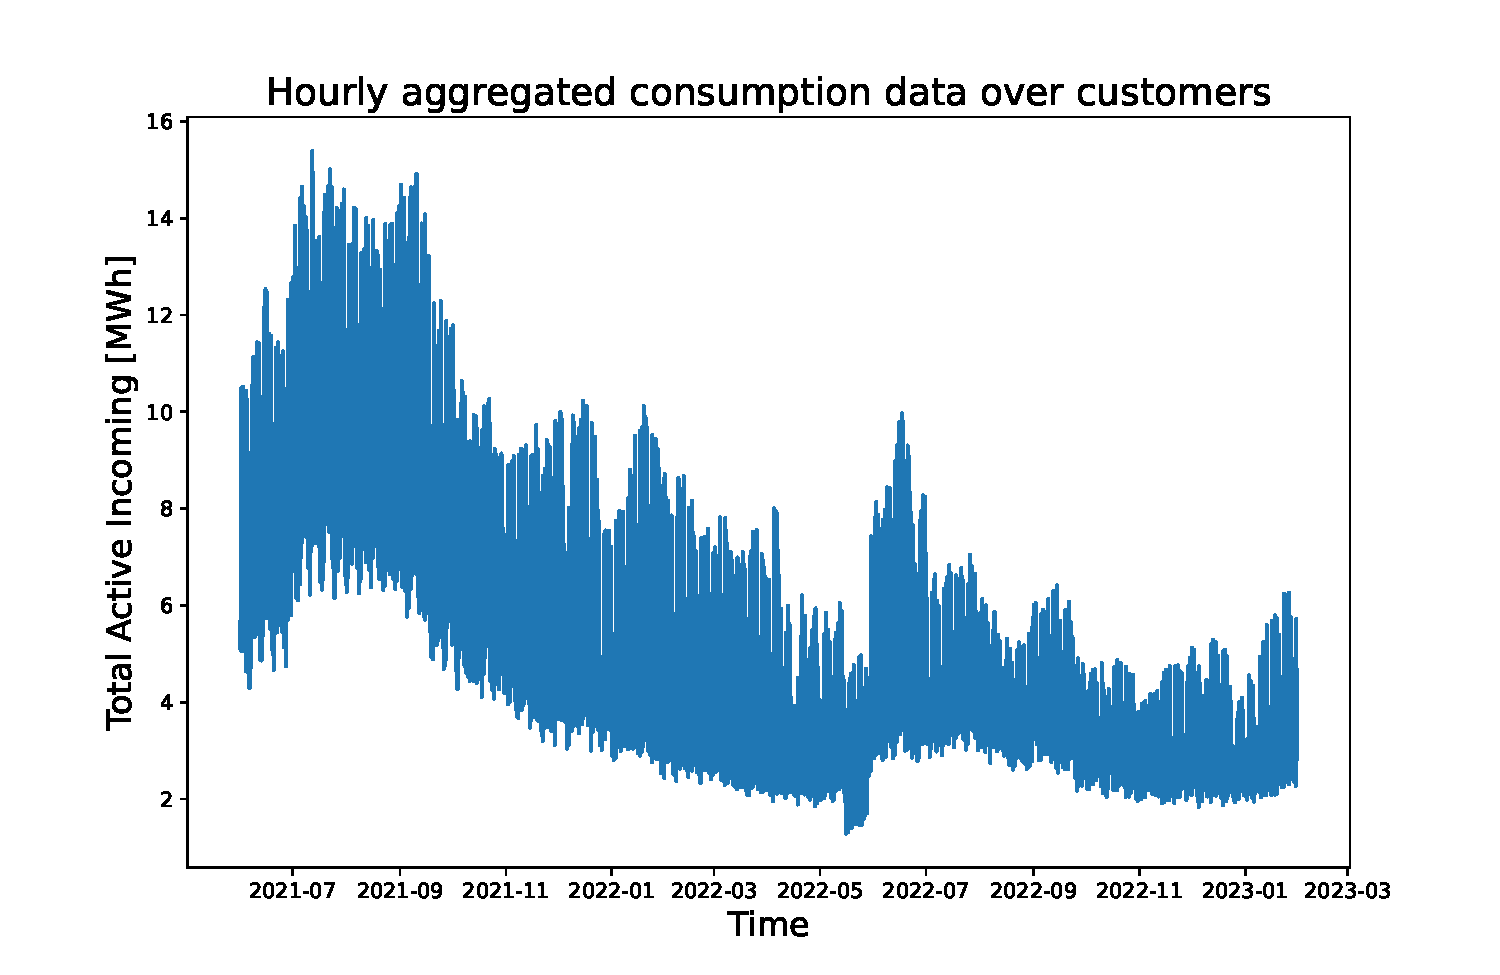
\includegraphics[width=1\textwidth]{images/demand/data_plot}
\subcaption{}
\label{fig:demanddataplot}
\end{minipage}
\ \hspace{2mm} \
\begin{minipage}[b]{8.5cm}
\centering
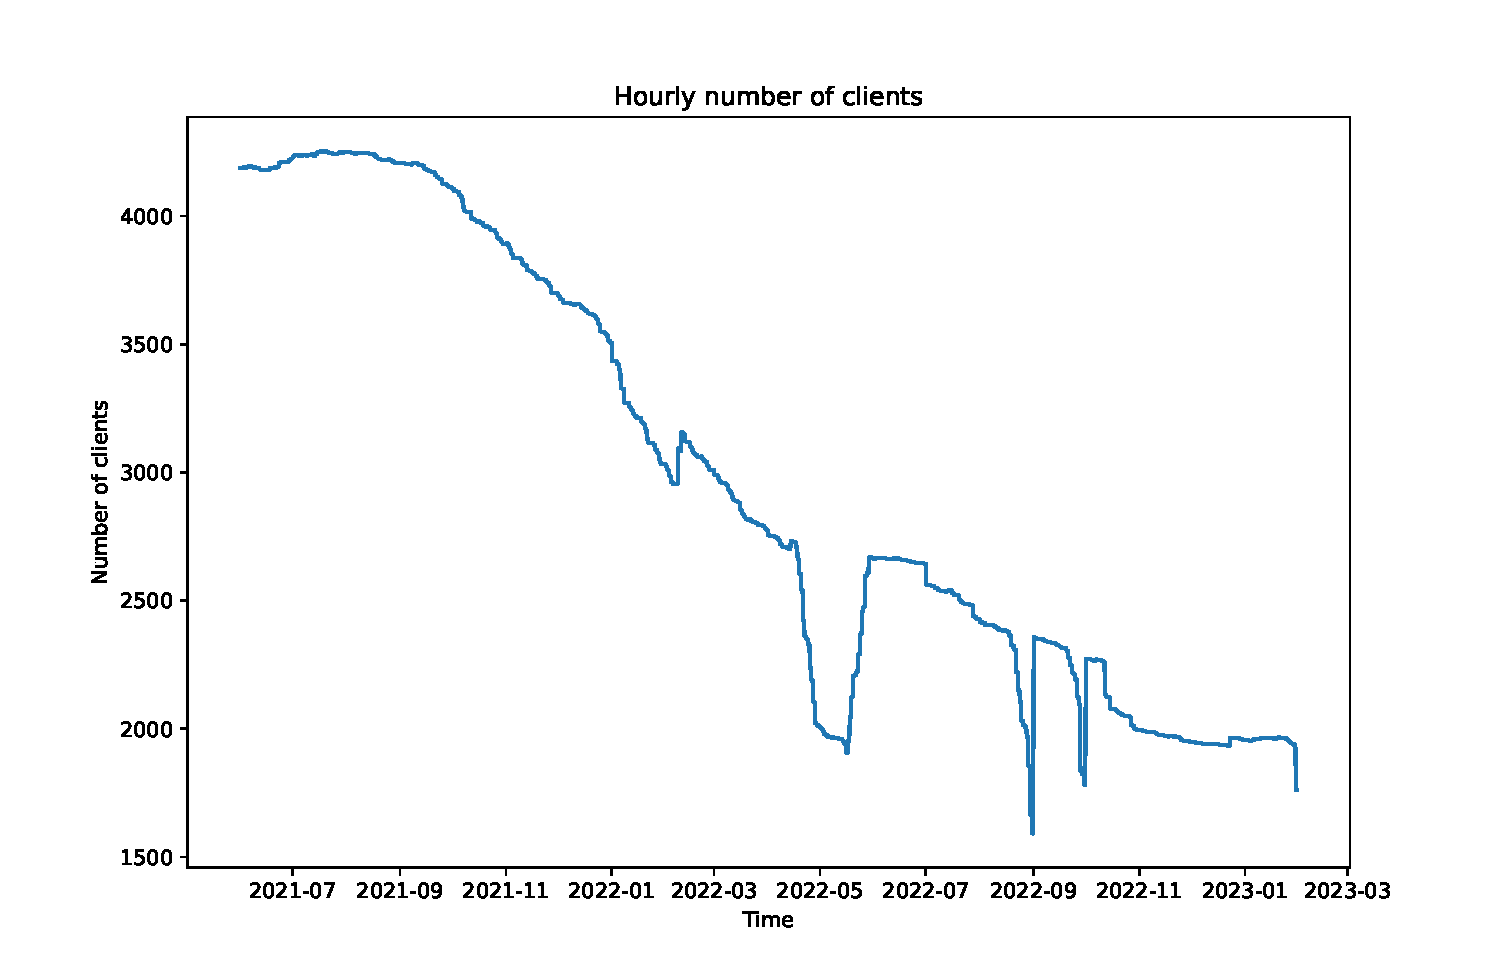
\includegraphics[width=1\textwidth]{images/demand/clients_plot}
\subcaption{}
\label{fig:clientsplot}
\end{minipage}
\begin{minipage}[b]{17cm}
\centering
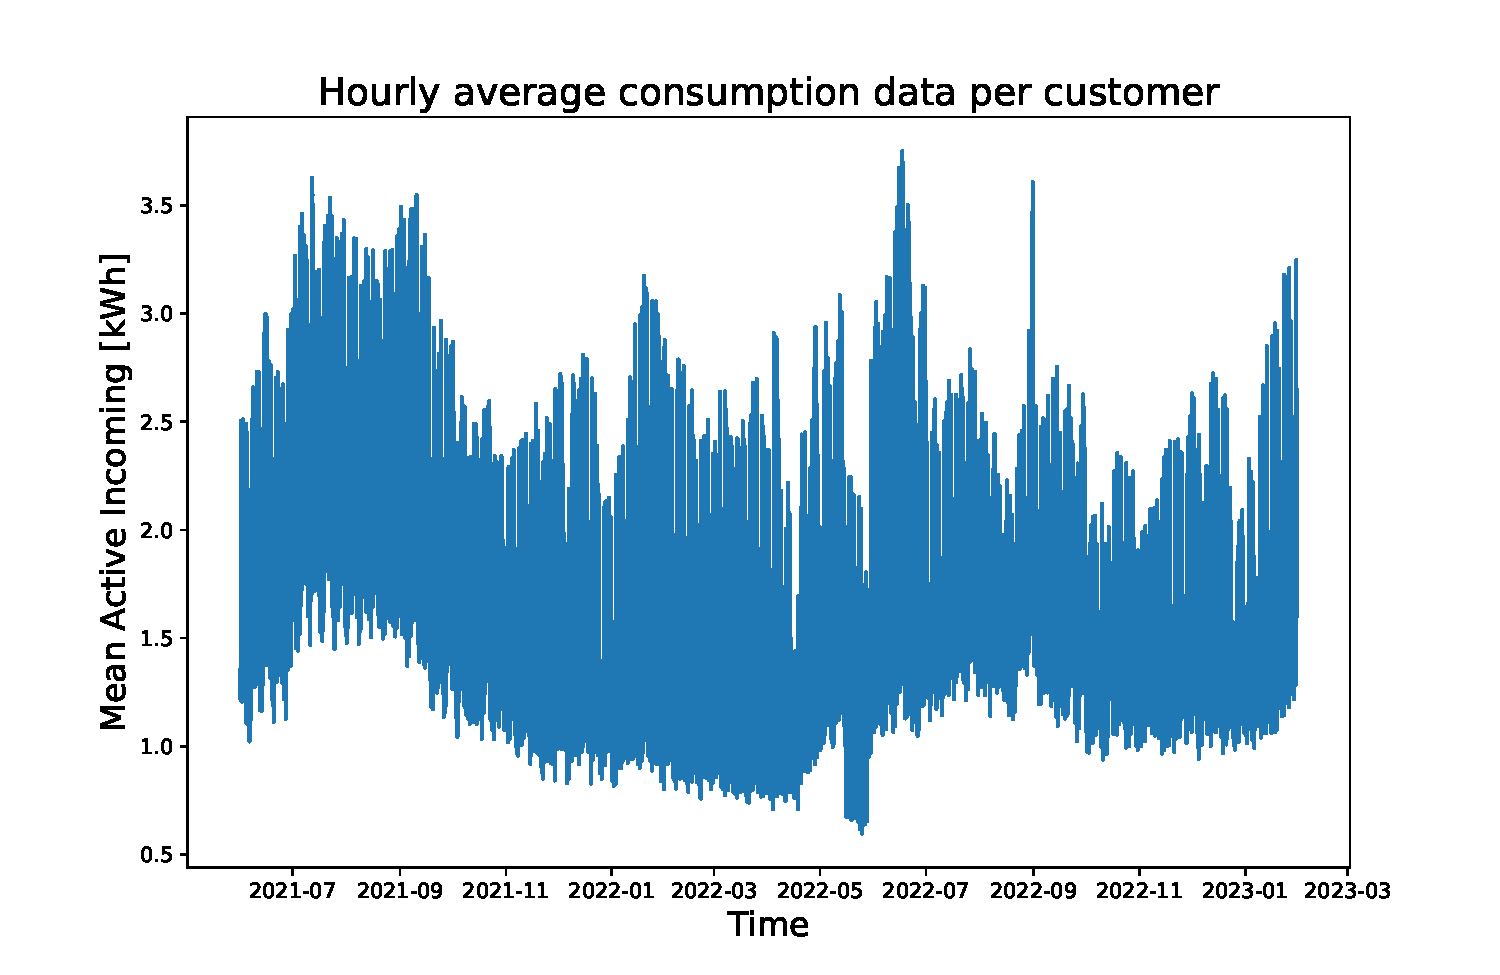
\includegraphics[width=0.5\textwidth]{images/demand/mean_data_plot}
\subcaption{}
\label{fig:meandemanddataplot}
\end{minipage}
\caption{The graphical representation of the hourly \subref{fig:demanddataplot} aggregated consumption data, \subref{fig:clientsplot} the number of clients, and \subref{fig:meandemanddataplot} the mean consumption data over the clients.}
\end{figure}

The aggregated consumption data from all their customers consists of hourly aggregated consumption data from June 2021 to January 2023 for a total of 14617 entries.
The graphical representation of the hourly aggregated consumption data is reported in figure~\ref{fig:demanddataplot}.
The number of customers is variable, with a maximum of 4253, a minimum of 1591, a mean of 2988, and a standard deviation of 855.
The graphical representation of the hourly number of clients is reported in figure~\ref{fig:clientsplot}.
It was thought to normalize the consumption on the number of customers for studying a kind of mean consumption per user as reported in figure~\ref{fig:meandemanddataplot} and then multiplying by the number of users, but this was not possible since often this value has a high change without reflecting on the consumption data, this information was not used since classified as unreliable.
Anyway, this mean value suggests the presence of two consumption peaks, one in summer, probably due to air conditioning systems, and the second one in winter, probably due to heating systems.

The consumption data from single customers consists of hourly aggregated consumption data of 4 customers:
\begin{enumerate}
  \item from June 2021 to May 2022 for a total of 8750 total entries (represented in figure~\ref{fig:dataplotcustomer1});
  \item from September 2021 to May 2022 for a total of 5855 total entries (represented in figure~\ref{fig:dataplotcustomer2});
  \item from September 2021 to August 2022 for a total of 8745 total entries (represented in figure~\ref{fig:dataplotcustomer3});
  \item from September 2021 to August 2022 for a total of 8760 total entries (represented in figure~\ref{fig:dataplotcustomer4}).
\end{enumerate}
The total entries for the 4 customers are 32110 in the overall period from June 2021 to August 2022.

\begin{figure}[H]
\begin{minipage}[b]{8.5cm}
\centering
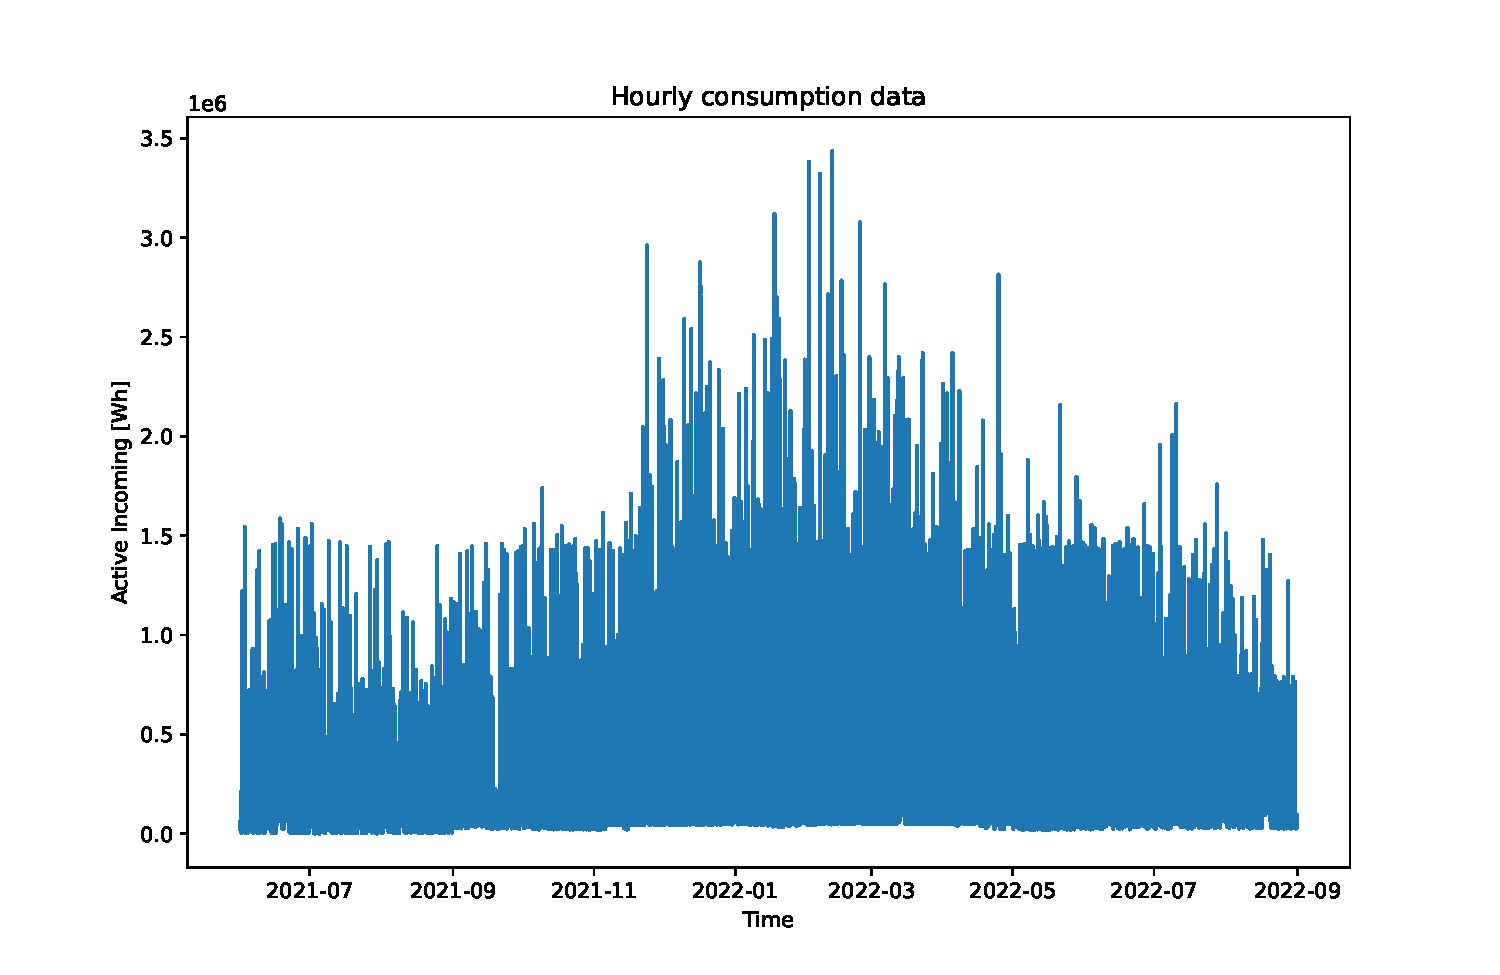
\includegraphics[width=1\textwidth]{images/baseline/data_plot_customer1}
\subcaption{First customer.}
\label{fig:dataplotcustomer1}
\end{minipage}
\ \hspace{2mm} \
\begin{minipage}[b]{8.5cm}
\centering
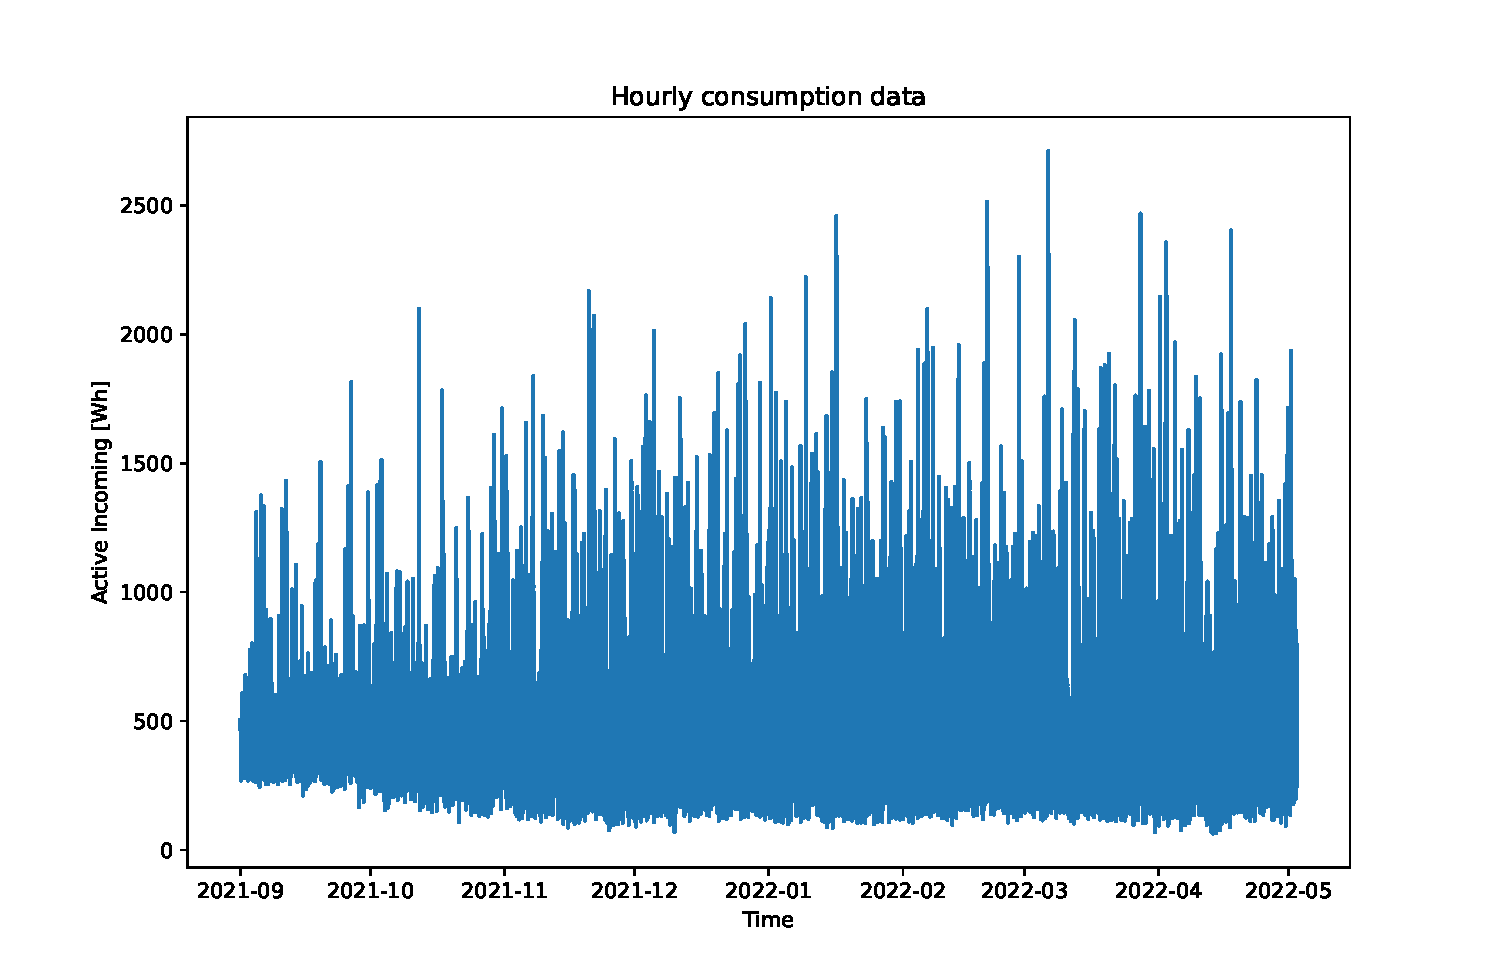
\includegraphics[width=1\textwidth]{images/baseline/data_plot_customer2}
\subcaption{Second customer.}
\label{fig:dataplotcustomer2}
\end{minipage}
\begin{minipage}[b]{8.5cm}
\centering
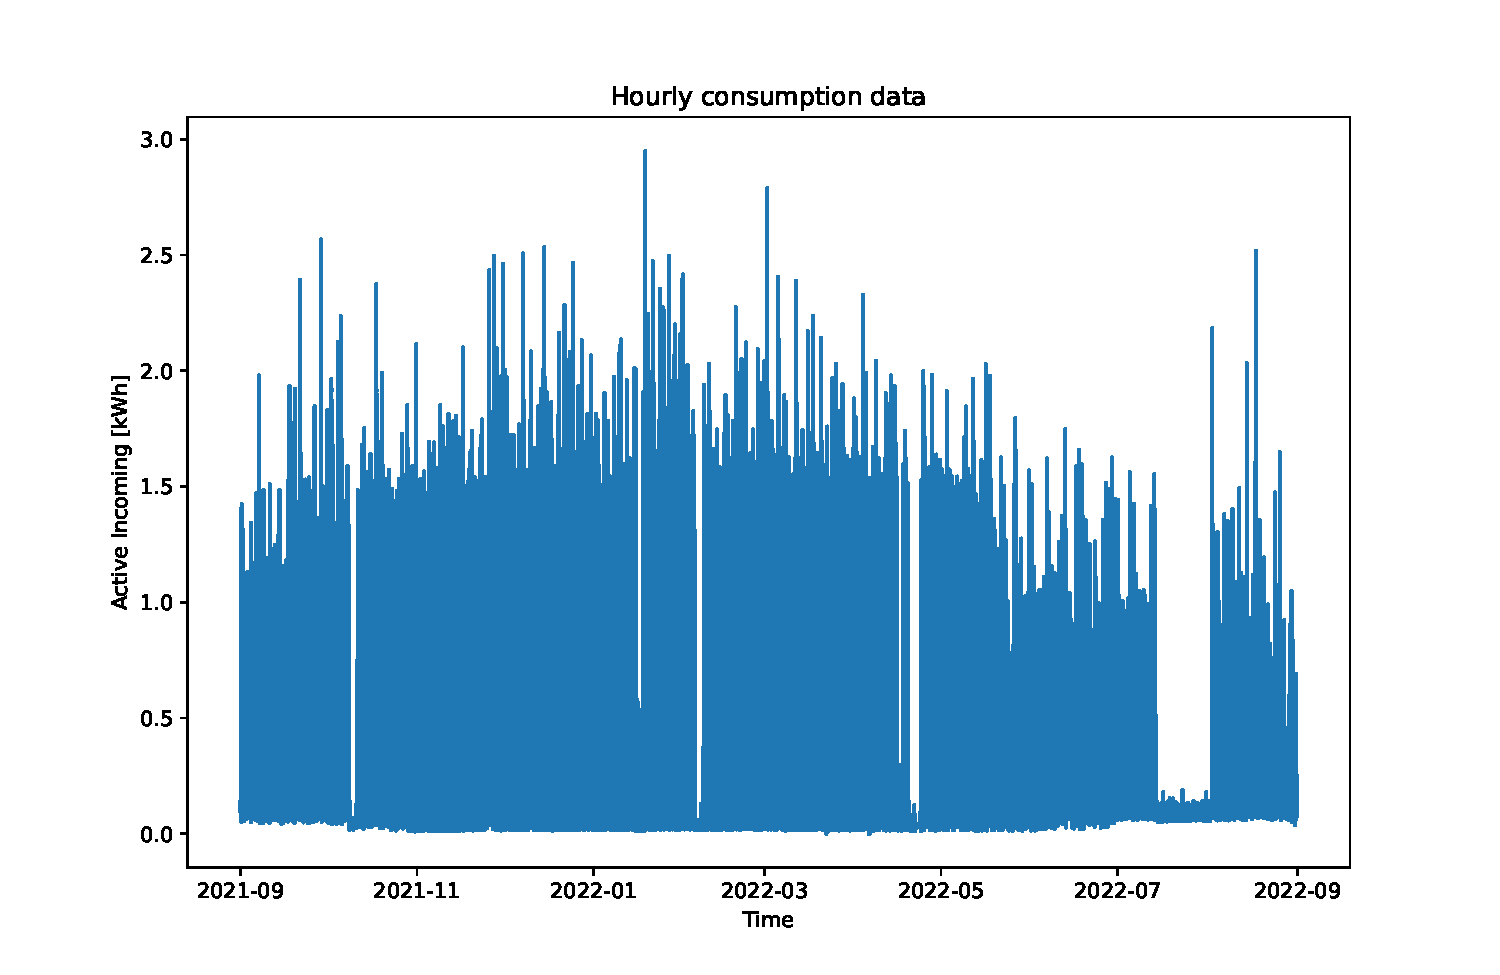
\includegraphics[width=1\textwidth]{images/baseline/data_plot_customer3}
\subcaption{Third customer.}
\label{fig:dataplotcustomer3}
\end{minipage}
\ \hspace{2mm} \
\begin{minipage}[b]{8.5cm}
\centering
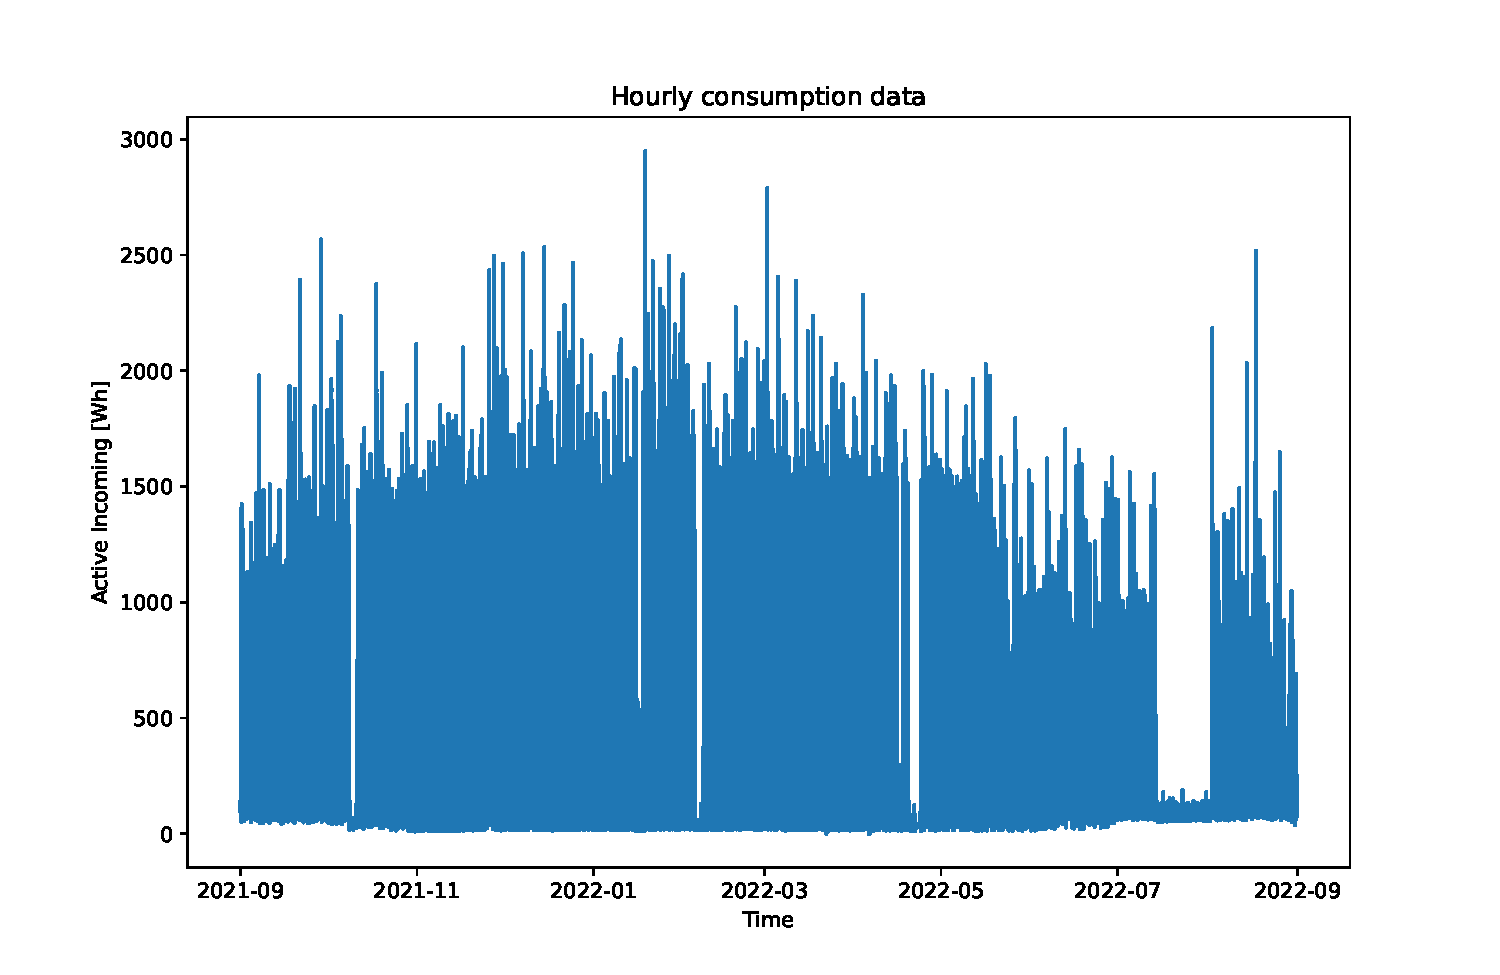
\includegraphics[width=1\textwidth]{images/baseline/data_plot_customer4}
\subcaption{Fourth customer.}
\label{fig:dataplotcustomer4}
\end{minipage}
\caption{The graphical representation of the consumption data of the 4 customers.}
\end{figure}

Just data of 4 customers were provided since consumption data of customers are considered as personal data as stated in the Directive (EU) 2019/944 of the European Parliament\footnote{ \url{https://eur-lex.europa.eu/legal-content/EN/TXT/?uri=CELEX:32019L0944} } that deals with common rules for the internal market for electricity.
So, energy data as personal data would be in accordance with the General Data Protection Regulation (GDPR)\footnote{ \url{https://gdpr-info.eu/} } and explicit consent for processing it is needed.
So they probably provided data of MIWEnergia internal workers that want to collaborate with the research.
In fact, some habitations were needed for a technical feasibility study but with data of more customers, it would be better to have more data and take into consideration possible consumption patterns of more customers.

From the data plots, it is possible to notice that these customer consumption data series have quite different patterns, for example:
\begin{itemize}
  \item The first and third customers, stay always under 1.5 kWh during the year except in the winter period;
  \item The second customer has almost the same consumption;
  \item The fourth customer has a dense series with some holes with very low consumption in parts of the year, probably due to periods out from home.
\end{itemize}

The production data from 8 PV plants consists of hourly aggregated production data:
\begin{enumerate}
  \item from January 2022 to October 2022 for a total of 7296 total entries and it has a nominal power of 149.75 kW;
  \item from February 2022 to October 2022 for a total of 6552 total entries and it has a nominal power of 237.6 kW;
  \item from February 2022 to October 2022 for a total of 6552 total entries and it has a nominal power of 158.4 kW;
  \item from June 2022 to October 2022 for a total of 3576 total entries and it has a nominal power of 1240 kW;
  \item from September 2022 to October 2022 for a total of 1465 total entries and it has a nominal power of 126.2 kW;
  \item from September 2022 to October 2022 for a total of 1465 total entries and it has a nominal power of 113 kW;
  \item from September 2022 to October 2022 for a total of 1465 total entries and it has a nominal power of 45 kW;
  \item from September 2022 to October 2022 for a total of 1465 total entries and it has a nominal power of 100 kW;
\end{enumerate}
The total entries for the 8 PV plants are 29836 total entries in the overall period from January 2022 to October 2022.
The graphical representation of the hourly aggregated total and mean percentage production data are reported respectively in figure~\ref{fig:productiondataplot} and figure~\ref{fig:productiondataplotpercentage}.

\begin{figure}[H]
\begin{minipage}[b]{8.5cm}
\centering
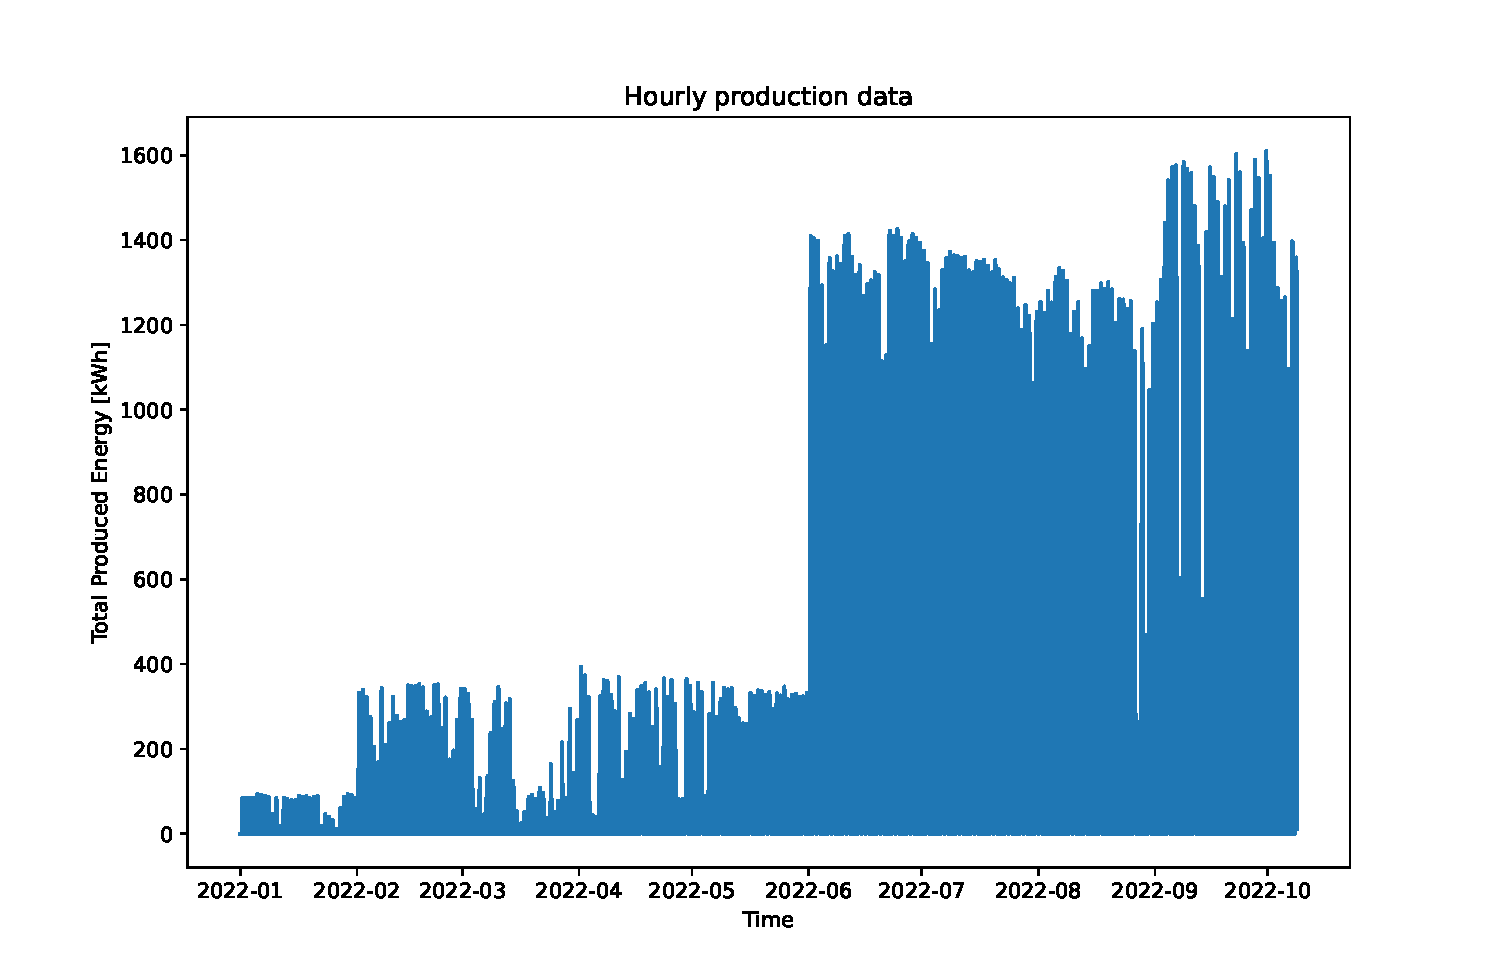
\includegraphics[width=1\textwidth]{images/production/data_plot}
\subcaption{}
\label{fig:productiondataplot}
\end{minipage}
\ \hspace{2mm} \
\begin{minipage}[b]{8.5cm}
\centering
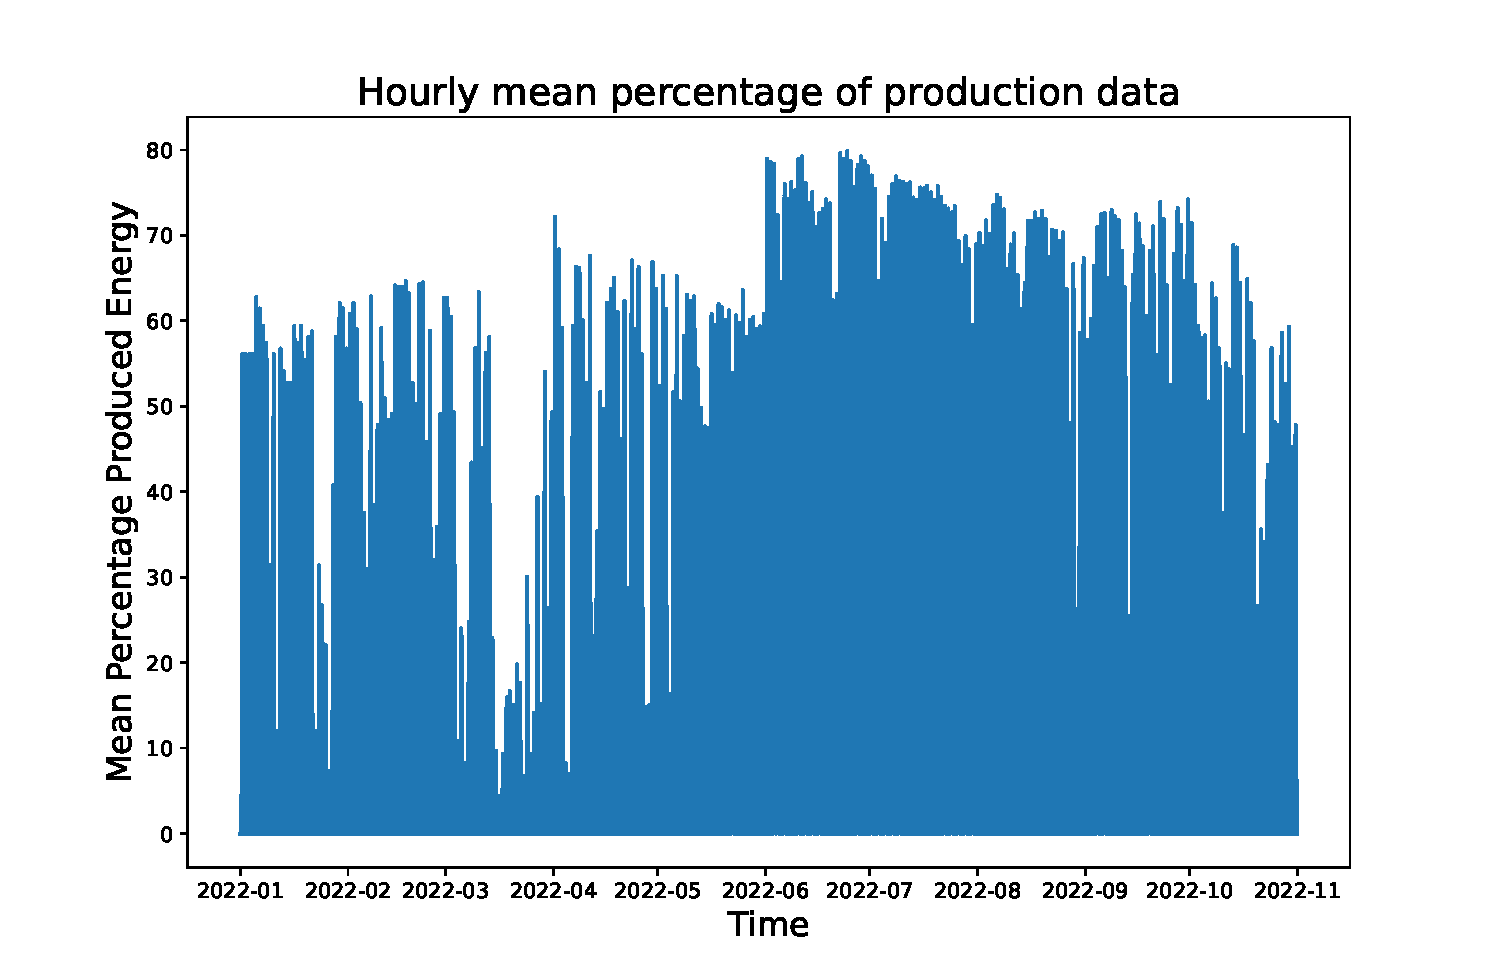
\includegraphics[width=1\textwidth]{images/production/data_plot_percentage}
\subcaption{}
\label{fig:productiondataplotpercentage}
\end{minipage}
\caption{The graphical representation of the hourly aggregated \subref{fig:umlsingleplant} total and \subref{fig:umlsingleplant} mean percentage production data.}
\end{figure}

The same weather data from the same provider and the same weather station were used for all the tasks, this was done since the customers and the PV plants were in the same area, with a maximum distance of the PV plants of around 100 km.


\section{Evaluation methodology}
\label{sec:methodology}
\vspace{0.2 cm}

The evaluation methodology was based on two relevant error metrics:
\begin{itemize}
  \item Mean Absolute Percentage Error (MAPE) is defined as $\text{MAPE}(y, \hat{y}) = \frac{100\%}{N} \sum_{i=0}^{N - 1} \frac{|y_i - \hat{y}_i|}{|y_i|}$. It is the most relevant error metric for all the tasks since it percentage-based error metric that takes into account the magnitude of the errors relative to the actual values.
  \item Mean Absolute Error (MAE) is defined as $\text{MAE}(y, \hat{y}) = \frac{ \sum_{i=0}^{N - 1} |y_i - \hat{y}_i| }{N}$. It is the most applicable error metric in consumption baseline forecasting where there is a high variability passing from very low to high values, and electricity production forecasting where there are a lot of zeros when the sun is not present.
\end{itemize}

Describe how the test of the performance of the models works ...

Treat the validation: describe the blocked k-fold validation and the hold-out approach repeated in multiple periods ...


\section{Electricity demand forecasting}
\label{sec:demandval}
\vspace{0.2 cm}

Analyze the data (descriptive analytics) and the results of the models for the electricity demand forecasting task (predictive analytics) ...

Data stats and correlation with weather data ...

Basic data is enhanced with the air temperature, the apparent temperature, and the relative humidity.

Describe the choice of parameters for models ... (list with motivations)

Summary table with results ...
% TODO where results are the one given by cross validation mean ± std


\section{Electricity production forecasting}
\label{sec:productionval}
\vspace{0.2 cm}

Analyze the data (descriptive analytics) and the results of the models for the electricity production forecasting task (predictive analytics) ...

As described in the data preprocessing in chapter~\ref{cha:implementation}, single PV plant production data are aggregated to obtain the aggregated production data over the PV plants.
The target of the predictions is the mean percentage of production, which is calculated as the division of the total produced energy by the total power of the PV plants.
This allows to have a bounded value from 0 to 100 from which it is possible to obtain the total produced energy simply by multiplying it by the total power of the PV plants.
(This was also done since plants are added over time and this was unpredictable, this results in predicting the percentage of production of the PV plants.)

Data stats and correlation with weather data ...

Basic data is enhanced with the air temperature, the apparent temperature, the relative humidity, the wind speed, the wind direction, the pressure altimeter, the visibility, the sky coverage, the diffuse horizontal irradiance, the direct normal irradiance, the global horizontal irradiance, the solar radiation, the UV index, the solar elevation angle, and the solar azimuth angle.
Only the hourly granularity is considered since PV plants are highly correlated with weather data and the aggregation over the day loses this correlation.
Probably if we were dealing with forecasting the production of each plant in isolation, the weather data at the specific locations of the plants can be used for achieving more accurate results and higher correlations, but since we are aggregating over them and looking for a percentage of production in the hour, the weather data from a location in the middle with respect to them is also acceptable.

Describe the choice of parameters for models ... (list with motivations)

Summary table with results ...
% TODO where results are the one given by cross validation mean ± std


\section{Consumption baseline forecasting} 
\label{sec:baselineval}
\vspace{0.2 cm}

Analyze the data (descriptive analytics) and the results of the models for the consumption baseline forecasting task (predictive analytics) ...

Data stats and correlation with weather data ...

As can be noticed from the data, there is high variability in consumption and low auto-correlation, this suggests how it is difficult to produce highly accurate results on a single customer level.
With just the time series of a few users, it is very difficult to learn a well-performing model, having more users it could be possible to learn certain generic trends or standard behaviors.

Basic data is enhanced with the air temperature, the apparent temperature, and the relative humidity.

Describe the choice of parameters for models ... (list with motivations)

Summary table with results ...
% TODO where results are the one given by cross validation mean ± std
